\documentclass[a4paper]{article}

\usepackage{tikz}
\usetikzlibrary{positioning, arrows.meta, shapes, calc}
\usepackage{float}
\usepackage{geometry}
\geometry{margin=1.5cm, landscape}

\begin{document}

\title{System Overview: Nuevo Pipeline Architecture}
\author{}
\date{}
\maketitle

\section{System Overview}

This diagram illustrates the detailed architecture of the \texttt{nuevo} pipeline, showing internal processing steps and data flows for both main components.

\begin{figure}[H]
  \centering
  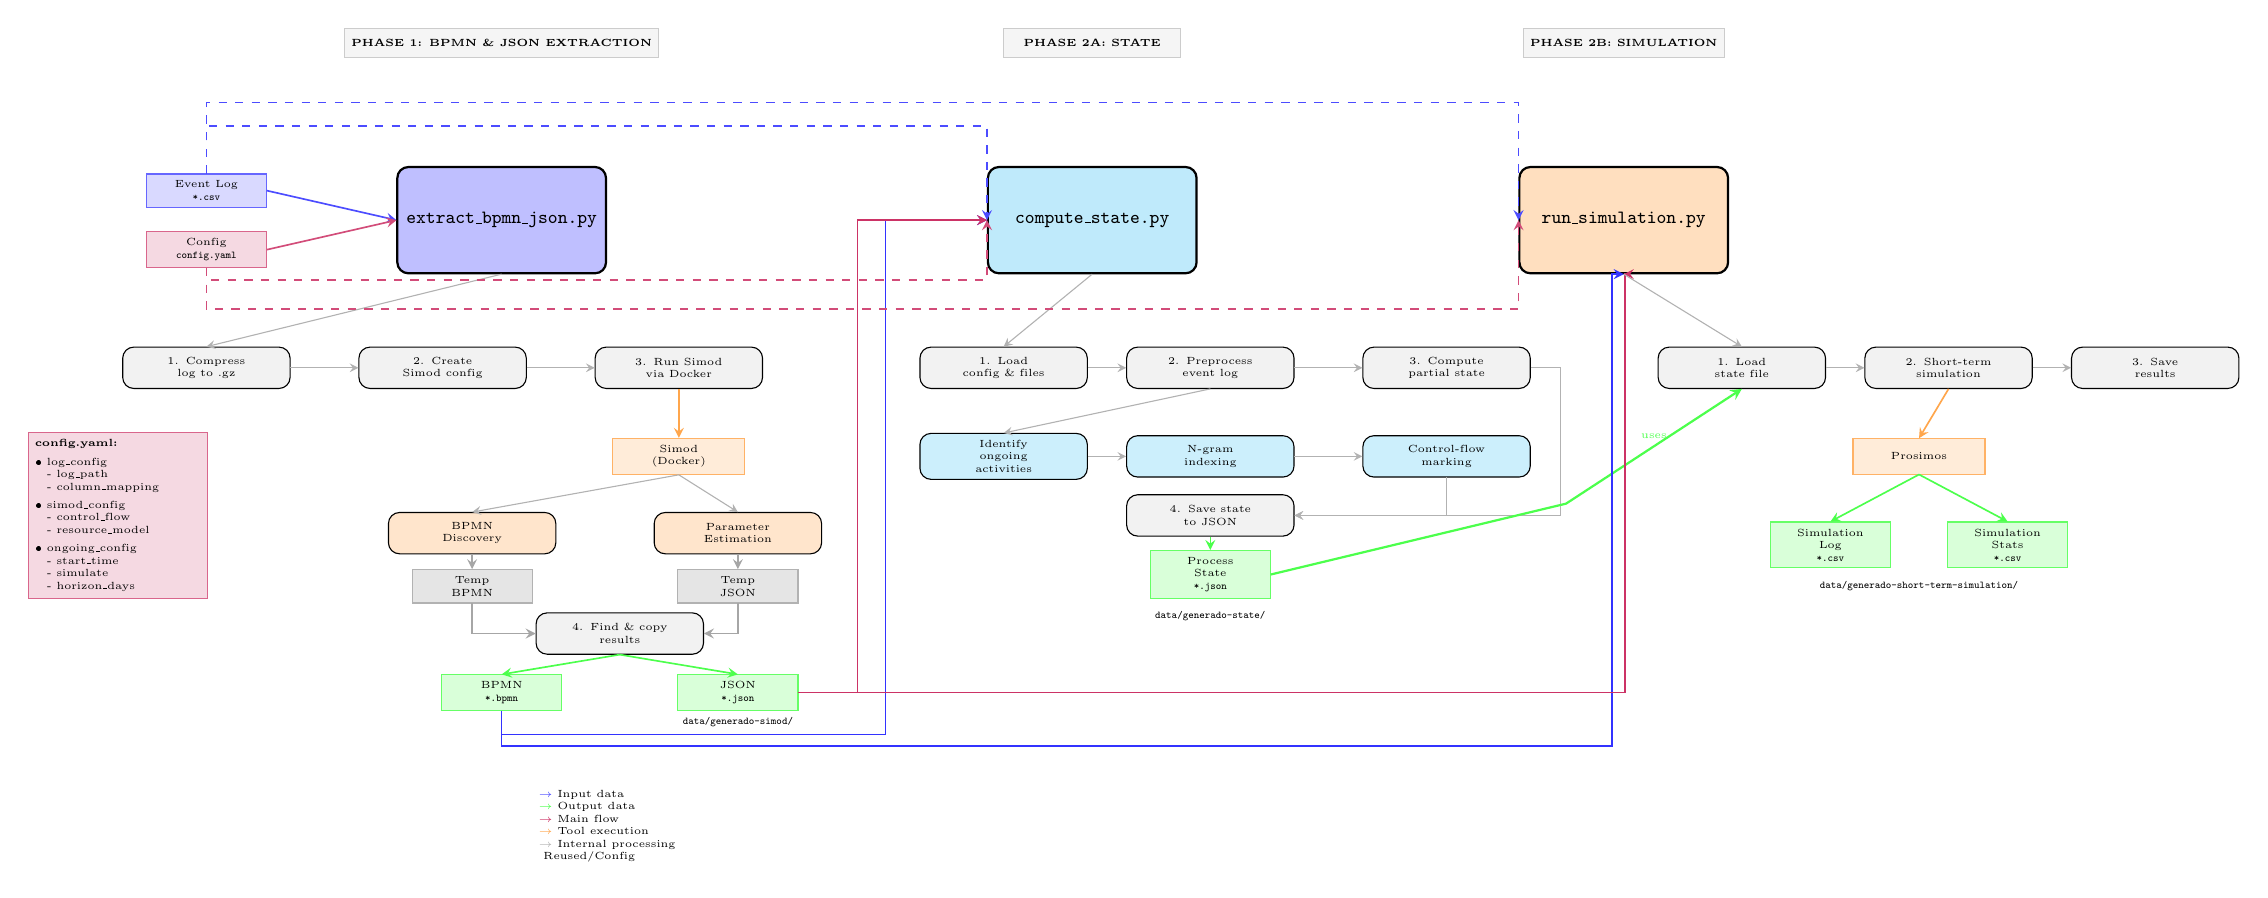
\begin{tikzpicture}[
    scale=0.75,
    transform shape,
    node distance=0.8cm and 1.5cm,
    script/.style={rectangle, rounded corners, draw=black, thick, 
                   minimum width=3.5cm, minimum height=1.8cm, 
                   text width=3.3cm, align=center, font=\small\bfseries},
    procstep/.style={rectangle, rounded corners, draw=black, fill=gray!10,
                 minimum width=2.8cm, minimum height=0.7cm,
                 text width=2.6cm, align=center, font=\tiny},
    input/.style={rectangle, draw=blue!60, fill=blue!15, 
                  minimum width=2cm, minimum height=0.5cm, 
                  text width=1.8cm, align=center, font=\tiny},
    output/.style={rectangle, draw=green!60, fill=green!15, 
                   minimum width=2cm, minimum height=0.5cm, 
                   text width=1.8cm, align=center, font=\tiny},
    config/.style={rectangle, draw=purple!60, fill=purple!15, 
                   minimum width=2cm, minimum height=0.5cm, 
                   text width=1.8cm, align=center, font=\tiny},
    tool/.style={rectangle, draw=orange!60, fill=orange!15,
                 minimum width=2.2cm, minimum height=0.6cm,
                 text width=2cm, align=center, font=\tiny},
    arrow/.style={->, >=stealth, semithick},
    phase/.style={rectangle, draw=gray!40, fill=gray!8, 
                  minimum width=3cm, minimum height=0.5cm, 
                  font=\tiny\bfseries, align=center},
    internal/.style={->, >=stealth, thin, gray!60}
  ]
    
    % Phase labels at top
    \node[phase] (phase1) at (-8, 8) {PHASE 1: BPMN \& JSON EXTRACTION};
    \node[phase] (phase2a) at (2, 8) {PHASE 2A: STATE};
    \node[phase] (phase2b) at (11, 8) {PHASE 2B: SIMULATION};
    
    % ========== PHASE 1 DETAILS ==========
    
    % Inputs to Phase 1
    \node[input] (log) at (-13, 5.5) {Event Log\\\texttt{*.csv}};
    \node[config] (config) at (-13, 4.5) {Config\\\texttt{config.yaml}};
    
    % extract_bpmn_json.py main module
    \node[script, fill=blue!25] (extract) at (-8, 5) {
      \texttt{extract\_bpmn\_json.py}
    };
    
    % Internal steps of extract_bpmn_json.py
    \node[procstep] (compress) at (-13, 2.5) {1. Compress\\log to .gz};
    \node[procstep] (create-config) at (-9, 2.5) {2. Create\\Simod config};
    \node[procstep] (docker) at (-5, 2.5) {3. Run Simod\\via Docker};
    
    % Simod tool
    \node[tool] (simod) at (-5, 1) {Simod\\(Docker)};
    
    % Simod internal processes
    \node[procstep, fill=orange!20] (discover) at (-8.5, -0.3) {BPMN\\Discovery};
    \node[procstep, fill=orange!20] (params) at (-4, -0.3) {Parameter\\Estimation};
    
    % Temporary outputs from Simod
    \node[output, draw=gray!60, fill=gray!20] (temp-bpmn) at (-8.5, -1.2) {Temp\\BPMN};
    \node[output, draw=gray!60, fill=gray!20] (temp-json) at (-4, -1.2) {Temp\\JSON};
    
    % Step 4: Copy results
    \node[procstep] (copy) at (-6, -2) {4. Find \& copy\\results};
    
    % Final outputs from Phase 1
    \node[output] (bpmn) at (-8, -3) {BPMN\\\texttt{*.bpmn}};
    \node[output] (json) at (-4, -3) {JSON\\\texttt{*.json}};
    
    % Output directory label
    \node[font=\tiny, align=center] at (-4, -3.5) {\texttt{data/generado-simod/}};
    
    % ========== PHASE 2A: STATE COMPUTATION ==========
    
    % compute_state.py main module
    \node[script, fill=cyan!25] (compute-state) at (2, 5) {
      \texttt{compute\_state.py}
    };
    
    % Internal steps of compute_state.py
    \node[procstep] (load) at (0.5, 2.5) {1. Load\\config \& files};
    \node[procstep] (preprocess) at (4, 2.5) {2. Preprocess\\event log};
    \node[procstep] (state) at (8, 2.5) {3. Compute\\partial state};
    
    % State computation details
    \node[procstep, fill=cyan!20] (ongoing-act) at (0.5, 1) {Identify\\ongoing\\activities};
    \node[procstep, fill=cyan!20] (n-gram) at (4, 1) {N-gram\\indexing};
    \node[procstep, fill=cyan!20] (marking) at (8, 1) {Control-flow\\marking};
    
    % Step 4: Save state JSON
    \node[procstep] (save-state) at (4, 0) {4. Save state\\to JSON};
    
    % State output
    \node[output] (state-json) at (4, -1) {Process\\State\\\texttt{*.json}};
    
    % Output directory label for state
    \node[font=\tiny, align=center] at (4, -1.7) {\texttt{data/generado-state/}};
    
    % ========== PHASE 2B: SIMULATION ==========
    
    % run_simulation.py main module
    \node[script, fill=orange!25] (run-sim) at (11, 5) {
      \texttt{run\_simulation.py}
    };
    
    % Internal steps of run_simulation.py
    \node[procstep] (load-state) at (13, 2.5) {1. Load\\state file};
    \node[procstep] (simulate) at (16.5, 2.5) {2. Short-term\\simulation};
    \node[procstep] (save-sim) at (20, 2.5) {3. Save\\results};
    
    % Prosimos tool
    \node[tool] (prosimos) at (16, 1) {Prosimos};
    
    % Simulation outputs
    \node[output] (sim-log) at (14.5, -0.5) {Simulation\\Log\\\texttt{*.csv}};
    \node[output] (sim-stats) at (17.5, -0.5) {Simulation\\Stats\\\texttt{*.csv}};
    
    % Output directory label for simulation
    \node[font=\tiny, align=center] at (16, -1.2) {\texttt{data/generado-short-term-simulation/}};
    
    % ========== ARROWS PHASE 1 ==========
    
    % Inputs to extract_bpmn_json.py
    \draw[arrow, blue!70] (log.east) -- (extract.west);
    \draw[arrow, purple!70] (config.east) -- (extract.west);
    
    % Internal flow in extract_bpmn_json.py
    \draw[internal] (extract.south) -- (compress.north);
    \draw[internal] (compress.east) -- (create-config.west);
    \draw[internal] (create-config.east) -- (docker.west);
    \draw[arrow, orange!70] (docker.south) -- (simod.north);
    
    % Simod internal
    \draw[internal] (simod.south) -- (discover.north);
    \draw[internal] (simod.south) -- (params.north);
    \draw[arrow, gray!70] (discover.south) -- (temp-bpmn.north);
    \draw[arrow, gray!70] (params.south) -- (temp-json.north);
    
    % Copy step
    \draw[arrow, gray!70] (temp-bpmn.south) |- (copy.west);
    \draw[arrow, gray!70] (temp-json.south) |- (copy.east);
    \draw[arrow, green!70] (copy.south) -- (bpmn.north);
    \draw[arrow, green!70] (copy.south) -- (json.north);
    
    % ========== ARROWS PHASE 2A: STATE ==========
    
    % Inputs to compute_state.py
    \draw[arrow, blue!70, dashed] (log.north) -- ++(0,0.8) -| (compute-state.west);
    \draw[arrow, purple!70, dashed] (config.south) -- ++(0,-0.2) -| (compute-state.west);
    \draw[arrow, blue!80] (bpmn.south) -- ++(0,-0.4) -- ++(6.5,0) |- (compute-state.west);
    \draw[arrow, purple!80] (json.east) -- ++(1,0) |- (compute-state.west);
    
    % Internal flow in compute_state.py
    \draw[internal] (compute-state.south) -- (load.north);
    \draw[internal] (load.east) -- (preprocess.west);
    \draw[internal] (preprocess.east) -- (state.west);
    
    % State computation details
    \draw[internal] (preprocess.south) -- (ongoing-act.north);
    \draw[internal] (ongoing-act.east) -- (n-gram.west);
    \draw[internal] (n-gram.east) -- (marking.west);
    \draw[internal] (marking.south) |- (save-state.east);
    \draw[internal] (state.east) -- ++(0.5,0) |- (save-state.east);
    \draw[arrow, green!70] (save-state.south) -- (state-json.north);
    
    % ========== ARROWS PHASE 2B: SIMULATION ==========
    
    % Inputs to run_simulation.py (state JSON from Phase 2A)
    \draw[arrow, green!70, thick] (state-json.east) -- ++(5,1.2) -- node[above, font=\tiny] {uses} (load-state.south);
    \draw[arrow, blue!80] (bpmn.south) -- ++(0,-0.6) -- ++(18.8,0) |- (run-sim.south);
    \draw[arrow, purple!80] (json.east) -- ++(14,0) |- (run-sim.south);
    \draw[arrow, blue!70, dashed] (log.north) -- ++(0,1.2) -| (run-sim.west);
    \draw[arrow, purple!70, dashed] (config.south) -- ++(0,-0.7) -| (run-sim.west);
    
    % Internal flow in run_simulation.py
    \draw[internal] (run-sim.south) -- (load-state.north);
    \draw[internal] (load-state.east) -- (simulate.west);
    \draw[internal] (simulate.east) -- (save-sim.west);
    
    % Simulation flow
    \draw[arrow, orange!70] (simulate.south) -- (prosimos.north);
    \draw[arrow, green!70] (prosimos.south) -- (sim-log.north);
    \draw[arrow, green!70] (prosimos.south) -- (sim-stats.north);
    
    % ========== CONFIGURATION DETAILS ==========
    
    % Config details box (left side)
    \node[config, minimum width=3cm, minimum height=2.5cm, 
          text width=2.8cm, align=left, font=\tiny] at (-14.5, 0) {
      \textbf{config.yaml:}\\
      \vspace{0.1cm}
      • log\_config\\
      \phantom{•} - log\_path\\
      \phantom{•} - column\_mapping\\
      \vspace{0.1cm}
      • simod\_config\\
      \phantom{•} - control\_flow\\
      \phantom{•} - resource\_model\\
      \vspace{0.1cm}
      • ongoing\_config\\
      \phantom{•} - start\_time\\
      \phantom{•} - simulate\\
      \phantom{•} - horizon\_days
    };
    
    % ========== LEGEND ==========
    \node[anchor=north west, font=\tiny] at (-7.5, -4.5) {
      \begin{tabular}{@{}l@{}}
        \textcolor{blue!70}{$\rightarrow$} Input data\\
        \textcolor{green!70}{$\rightarrow$} Output data\\
        \textcolor{purple!80}{$\rightarrow$} Main flow\\
        \textcolor{orange!70}{$\rightarrow$} Tool execution\\
        \textcolor{gray!60}{$\rightarrow$} Internal processing\\
        \textcolor{blue!70}{$\dashrightarrow$} Reused/Config
      \end{tabular}
    };
    
  \end{tikzpicture}
  \caption{Detailed architecture of the \texttt{nuevo} pipeline. 
           \textbf{Phase 1} (left): \texttt{extract\_bpmn\_json.py} compresses the event log, 
           creates Simod configuration, executes Simod via Docker for BPMN discovery and parameter 
           estimation, then copies results to \texttt{data/generado-simod/}. 
           \textbf{Phase 2A} (center): \texttt{compute\_state.py} loads configuration and files, 
           preprocesses the event log, computes partial process state (identifying ongoing activities, 
           building N-gram indices, computing control-flow markings), and saves the state to 
           \texttt{data/generado-state/}. 
           \textbf{Phase 2B} (right): \texttt{run\_simulation.py} loads the computed state, 
           executes short-term simulation via Prosimos using the partial state as initial condition, 
           and produces outputs in \texttt{data/generado-short-term-simulation/}.}
  \label{fig:architecture}
\end{figure}

\end{document}
